\ifdefined\beamerclass
\else
    \def\beamerclass{beamer}
\fi
\documentclass[\beamerclass]{beamer}

\usepackage{pgfpages}
\mode<handout>{
  % \setbeamercolor{background canvas}{bg=black!20}
  \pgfpagesuselayout{2 on 1}[a4paper,border shrink=5mm]
}

\usepackage[english]{babel}
\usepackage{algorithm}
\usepackage[noend]{algpseudocode}
\usepackage[utf8x]{inputenc}
\usepackage{graphicx}
\usepackage{hyperref}
%\graphicspath{{./images/}}
\usepackage{tikz}
\usetikzlibrary{shapes.geometric, arrows,chains}
\usepackage{booktabs,makecell,multirow,tabularx}
\usepackage{verbatim}
\renewcommand{\arraystretch}{1.2}
\renewcommand\theadfont{\normalfont\bfseries}
\usepackage{array}
\usepackage{listings}
\lstset{language=Java, showstringspaces=false}
\usepackage[normalem]{ulem}
\usepackage{bm}
\def\layersep{2.5cm}

\usepackage{xcolor}
%\usepackage{subfig}
\setbeamertemplate{caption}{\insertcaption}
\usepackage[caption=false]{subfig}
\usepackage{hyperref}
\usepackage{verbatim}
%\setbeamertemplate{caption}[numbered]%\numberwithin{figure}{section}
% Define block styles
\tikzstyle{decision} = [diamond, draw, fill=blue!20, 
    text width=4.5em, text badly centered, node distance=3cm, inner sep=0pt]
\tikzstyle{block} = [rectangle, draw, fill=blue!20, 
    text width=3em, text centered, rounded corners, minimum height=3em]
\tikzstyle{line} = [draw, -latex']
\tikzstyle{cloud} = [draw, ellipse, fill=red!20, node distance=3cm,
    minimum height=2em]
\tikzset{
  startstop/.style={
    rectangle, 
    rounded corners,
    minimum width=3cm, 
    minimum height=1cm,
    align=center, 
    draw=black, 
    fill=red!30
    },
  process/.style={
    rectangle, 
    minimum width=3cm, 
    minimum height=1cm, 
    align=center, 
    draw=black, 
    fill=blue!30
    },
  decision/.style={
    rectangle, 
    minimum width=3cm, 
    minimum height=1cm, align=center, 
    draw=black, 
    fill=green!30
    },
  arrow/.style={thick,->,>=stealth},
  dec/.style={
    ellipse, 
    align=center, 
    draw=black, 
    fill=green!30
    },
}
\tikzstyle{arrow} = [thick,->,>=stealth]

\tikzset{onslide/.code args={<#1>#2}{%
  \only<#1>{\pgfkeysalso{#2}} % \pgfkeysalso doesn't change the path
}}

\makeatletter
\newenvironment<>{btHighlight}[1][]
{\begin{onlyenv}#2\begingroup\tikzset{bt@Highlight@par/.style={#1}}\begin{lrbox}{\@tempboxa}}
{\end{lrbox}\bt@HL@box[bt@Highlight@par]{\@tempboxa}\endgroup\end{onlyenv}}

\newcommand<>\btHL[1][]{%
  \only#2{\begin{btHighlight}[#1]\bgroup\aftergroup\bt@HL@endenv}%
}
\def\bt@HL@endenv{%
  \end{btHighlight}%   
  \egroup
}
\newcommand{\bt@HL@box}[2][]{%
  \tikz[#1]{%
    \pgfpathrectangle{\pgfpoint{1pt}{0pt}}{\pgfpoint{\wd #2}{\ht #2}}%
    \pgfusepath{use as bounding box}%
    \node[anchor=base west, fill=orange!30,outer sep=0pt,inner xsep=1pt, inner ysep=0pt, rounded corners=3pt, minimum height=\ht\strutbox+1pt,#1]{\raisebox{1pt}{\strut}\strut\usebox{#2}};
  }%
}
\makeatother

\usepackage{amsmath}
\usepackage{mathdots}
\usepackage{yhmath}
\usepackage{cancel}
\usepackage{color}
\usepackage{siunitx}
\usepackage{array}
\usepackage{multirow}
\usepackage{amssymb}
\usepackage{gensymb}
\usepackage{tabularx}
\usepackage{booktabs}
\usetikzlibrary{fadings}
\usetikzlibrary{patterns}
\usetikzlibrary{shadows.blur}


\usetheme{Copenhagen}
\hypersetup{pdfstartview={Fit}}
\lstset{basicstyle=\small\ttfamily,breaklines=true}

\title[COMP6258]{Recap of Basic Neural Networks}
\subtitle{(and some Deep Network Fundamentals)}
\author{Jonathon Hare}
\institute[]
{
  Vision, Learning and Control\\
  University of Southampton 
}
\date{}
\subject{Computer Science}
\useoutertheme{infolines}
\setbeamertemplate{headline}{} %remove headline
\setbeamertemplate{navigation symbols}{} %remove navigation symbols

\definecolor{darkblue}{RGB}{37,55,97}
\definecolor{mellowyellow}{RGB}{247,206,70}
\definecolor{almostwhite}{RGB}{254,255,255}
\definecolor{merrygreen}{RGB}{79,173,91}

\addtobeamertemplate{footnote}{\hskip -2em}{}
\newcommand\blfootnote[1]{%
  \begingroup
  \renewcommand\thefootnote{}\footnote{#1}%
  \addtocounter{footnote}{-1}%
  \endgroup
}

\DeclareMathOperator{\softmax}{softmax}

\begin{document}

\begin{frame}[plain]
        \begin{tikzpicture}[overlay, remember picture, shift={(current page.south west)},font={\fontfamily{Montserrat-TOsF}\selectfont}]
        \fill [merrygreen,text=darkblue] (0,0) rectangle (\paperwidth, \paperheight);
        \draw (4,7) node [align=left,text=almostwhite] {\Huge \begin{tabular}{l} \textbf{Train,} \\ \textbf{Validate,} \\ \textbf{Test} \end{tabular}};
        \draw (11,1) node [align=left,text=almostwhite] {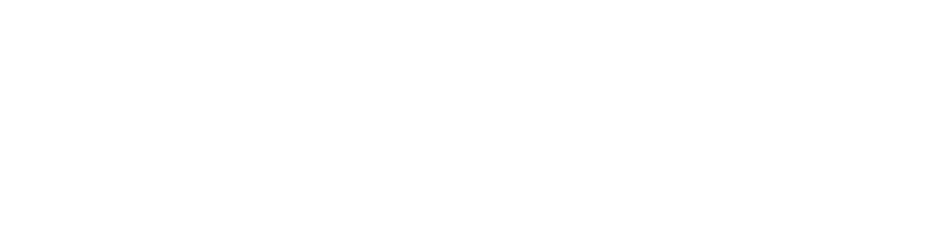
\includegraphics[scale=0.15]{../vlc.png}};
        \end{tikzpicture}
\end{frame}


\begin{frame}
  \titlepage
\end{frame}
%%-------------------------------------------------------------%

\begin{frame}[fragile]\frametitle{Classical Types of Learning}
\begin{itemize}
\item Supervised Learning - learn to predict an output when given an input vector

\item Unsupervised Learning - discover a good internal representation of the input

\item Reinforcement Learning - learn to select an action to maximize the expectation of future rewards (payoff)

\item Semi-supervised Learning - learn with few labelled examples and many unlabelled ones
\end{itemize}

\end{frame}

\begin{frame}[fragile]\frametitle{Other Types of Learning}
\begin{itemize}
\item Self-supervised Learning - learn with targets induced by a prior on the unlabelled training data

\item Active Learning - learn by seeking guidance from human or oracle when needed (iterative semi-supervised learning)

\item Continual Learning - learn new tasks/classes sequentially (iterative supervised/unsupervised learning)

\item Online learning - learning one example at a time sequentially (iterative supervised learning)
\end{itemize}

\end{frame}

%%-------------------------------------------------------------%

% \begin{frame}[fragile]\frametitle{Supervised Learning}
% \begin{center}
%   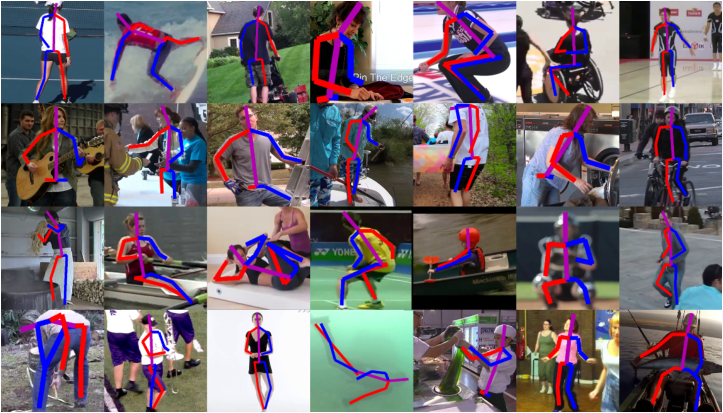
\includegraphics[width=.9\textwidth]{figs/SL.pdf}
%   \blfootnote{Newell, Alejandro, Kaiyu Yang, and Jia Deng. ``Stacked hourglass networks for human pose estimation.'' ECCV'16. Springer, 2016.}
% \end{center}
% \end{frame}
%%-------------------------------------------------------------%

% \begin{frame}[fragile]\frametitle{Unsupervised Learning}
% \begin{center}
%   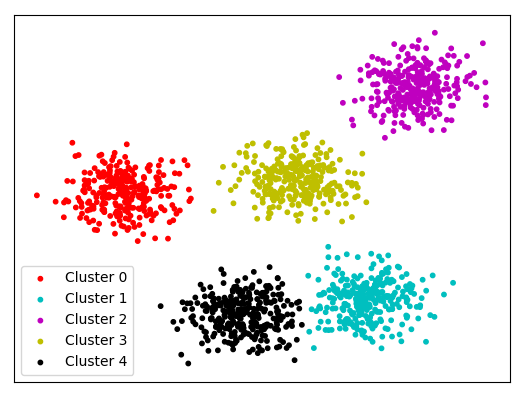
\includegraphics[width=0.8\textwidth]{figs/k-means.png}
% \end{center}
% \end{frame}
%%-------------------------------------------------------------%

% \begin{frame}[fragile]\frametitle{Reinforcement Learning}
% \begin{center}
%   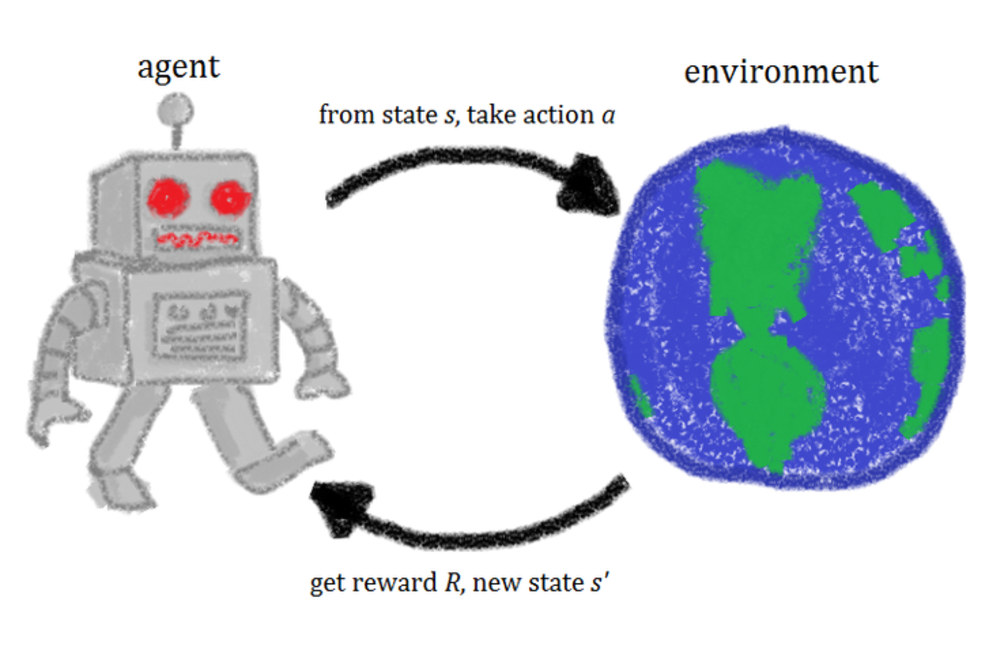
\includegraphics[width=0.9\textwidth]{figs/RL.pdf}
%   \blfootnote{Reference: Wikipedia \url{https://simple.wikipedia.org/wiki/Reinforcement_learning}}
% \end{center}
% \end{frame}
%%-------------------------------------------------------------%

% \begin{frame}[fragile]\frametitle{Self-supervised Learning}
% \begin{center}
%   \resizebox{0.8\textwidth}{!}{\input{figs/emecomm_model.tikz}\unskip}
%   \blfootnote{Daniela Mihai and Jonathon Hare. Avoiding hashing and encouraging visual semantics in referential emergent language games. EmeCom @ NeurIPS 2019. https://arxiv.org/abs/1911.05546}
% \end{center}

% \end{frame}
%%-------------------------------------------------------------%

% \begin{frame}[fragile]\frametitle{Semi-supervised Learning}
% \begin{center}
%  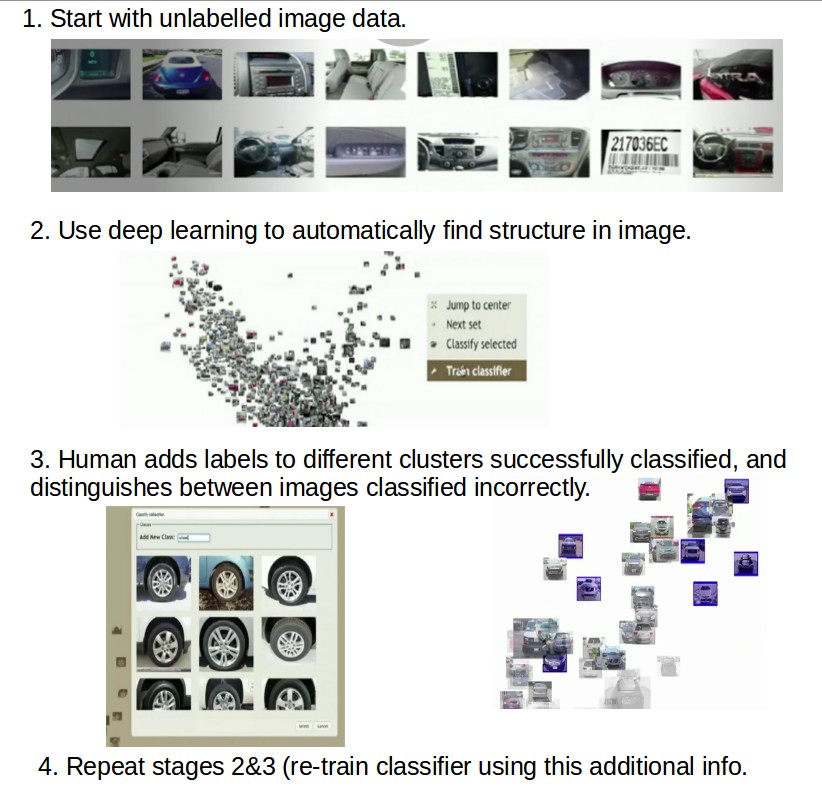
\includegraphics[width=0.6\textwidth]{figs/SS.png}\blfootnote{Jeremy Howard. The wonderful and terrifying implications of computers that can learn. TEDxBrussels. \url{http://www.ted.com/talks/jeremy_howard_the_wonderful_and_terrifying_implications_of_computers_that_can_learn}}
% \end{center}
% \end{frame}
%%-------------------------------------------------------------%

% \begin{frame}[fragile]\frametitle{Generative Models}
% \begin{itemize}
%   \item Many unsupervised and self-supervised models can be classed as `Generative Models'.
%   \item Given unlabelled data $X$, a unsupervised generative model learns $P[X]$.
%   \begin{itemize}
%     \item Could be direct modelling of the data (e.g. Gaussian Mixture Models)
%     \item Could be indirect modelling by learning to map the data to a parametric distribution in a lower dimensional space (e.g. a VAE's Encoder) or by learning a mapping from a parameterised distribution to the real data space (e.g. a VAE Decoder or GAN)
%   \end{itemize}
%   \item These are characterised by an ability to `sample' the model to `create' new data
% \end{itemize}
% %\url{http://robotics.stanford.edu/~ang/papers/nips01-discriminativegenerative.pdf}
% \end{frame}

%%-------------------------------------------------------------%

% \begin{frame}[fragile]\frametitle{Generative vs. Discriminative Models (II)}
% Generative vs. discriminative approaches to classification use different statistical modelling.
% \begin{itemize}
% \item Discriminative models learn the boundary between classes. A (probabilistic) discriminative model is a model of the conditional probability of the target $Y$ given an observation $X$: $P[Y|X]$.
% \item Generative models of labelled data model the distribution of individual classes. Given an observable variable $X$ and a target variable $Y$, a generative model is a statistical model that tries to model $P[X|Y]$ and $P[Y]$ in order to model the joint probability distribution $P[X, Y]$.\footnote{Some such models can be sampled conditionally based on a prior $Y$ - e.g. a Conditional VAE: \url{https://papers.nips.cc/paper/5775-learning-structured-output-representation-using-deep-conditional-generative-models}}
% \end{itemize} 

% % Additional Reading: \url{http://cs229.stanford.edu/notes/cs229-notes2.pdf}
% %\url{http://robotics.stanford.edu/~ang/papers/nips01-discriminativegenerative.pdf}
% \end{frame}

%%-------------------------------------------------------------%

\begin{frame}[fragile]\frametitle{Two Types of Supervised Learning}
\begin{itemize}
\item<+-> Regression:  The machine is asked predict $k$ numerical values given some input. The machine is a function $f: \mathbb{R}^n \rightarrow \mathbb{R}^k$.
\item<+-> Classification:  The machine is asked to specify which of $k$ categories some input belongs to.
\begin{itemize}
  \item Multiclass classification - target is one of the $k$ classes
  \item Multilabel classification - target is some number of the $k$ classes
  \item In both cases, the machine is a function $f : \mathbb{R}^n \rightarrow \{1, ..., k\}$.
\end{itemize}
\item<+-> It is most common for both types of algorithms to actually learn $\hat f : \mathbb{R}^n \rightarrow \mathbb{R}^k$.
\mode<article>{\item<+-> Note that there are lots of exceptions in the form the inputs (and outputs) can take though! We'll see lots of variations in the coming weeks.}
\end{itemize}
\end{frame}
%%-------------------------------------------------------------%


\begin{frame}[fragile]\frametitle{How Supervised Learning Typically Works}
\begin{itemize}
\item Start by choosing a model-class: $\hat y = f(\bm x; \bm W)$ where the model-class $f$ is a way of using some numerical parameters, $\bm W$, to map each input vector $\bm x$ to a predicted output $ \hat y$.
\item \emph{Learning} means adjusting the parameters to reduce the discrepancy between the true target output $y$ on each training case and the output $\hat y$, predicted by the model. %\footnote{Reference: Geoffrey Hinton \url{https://www.cs.toronto.edu/~hinton/coursera/lecture1/lec1e.mp4}}
\end{itemize}

\end{frame}

%%-------------------------------------------------------------%

\begin{frame}[fragile]\frametitle{Let's look at a Multilayer Perceptron (without biases)...}
  \begin{center}
    \begin{tikzpicture}[shorten >=1pt,->,draw=black!50, node distance=\layersep]
        \tikzstyle{every pin edge}=[<-,shorten <=1pt]
        \tikzstyle{neuron}=[circle,fill=black!25,minimum size=17pt,inner sep=0pt]
        \tikzstyle{input neuron}=[neuron, fill=green!50];
        \tikzstyle{output neuron}=[neuron, fill=red!50];
        \tikzstyle{hidden neuron}=[neuron, fill=blue!50];
        \tikzstyle{annot} = [text width=4em, text centered]

        % Draw the input layer nodes
        \foreach \name / \y in {1,...,4}
        % This is the same as writing \foreach \name / \y in {1/1,2/2,3/3,4/4}
            \node[input neuron] (I-\name) at (0,-\y) {$x_\y$};

        % Draw the hidden layer nodes
        \foreach \name / \y in {1,...,5}
            \path[yshift=0.5cm]
                node[hidden neuron] (H-\name) at (1.5*\layersep,-\y cm) {$h_\y$};

        % Draw the output layer node
            \foreach \name / \y in {1,...,2}
            \path[yshift=0.5cm]
                node[output neuron, pin={[pin edge={->}]right:$\hat y_\y$}, right of=H-3] (O-\name) at (1.5*\layersep,-40-\y cm) {$o_\y$};
        %\node[output neuron,pin={[pin edge={->}]right:Output}, right of=H-3] (O) {o};

        % Connect every node in the input layer with every node in the
        % hidden layer.
        \path (I-1) edge node[anchor=south] {$w_{ji}^{(1)}$}(H-1);
       \foreach \source in {1,...,4}
            \foreach \dest in {1,...,5}
           % \draw [arrow] (I-\source) - (H-\dest);
                \path (I-\source) edge (H-\dest) ;

        % Connect every node in the hidden layer with the output layer
        \path (H-1) edge node[anchor=south] {$w_{kj}^{(2)}$}(O-1);
        \foreach \source in {1,...,5}
           \foreach \dest in {1,...,2}
            \path (H-\source) edge (O-\dest);

        % Annotate the layers
        \node[annot,above of=H-1, node distance=1cm] (hl) {Hidden layer};
        \node[annot,left of=hl] {Input layer};
        \node[annot,right of=hl] {Output layer};
    \end{tikzpicture}
  \end{center}
  Without loss of generality, we can write the above as:
  \begin{center}
    $\hat{\bm y} = g(f(\bm x; \bm W^{(1)}); \bm W^{(2)}) = g(\bm{W}^{(2)} f(\bm{W}^{(1)} \bm x))$\\
  \end{center}
  where $f$ and $g$ are activation functions.
\end{frame}

%%-------------------------------------------------------------%
\begin{frame}[fragile]\frametitle{Common Activation Functions}

\begin{itemize}
  \item Identity
  \item Sigmoid (aka Logistic)
  \item Hyperbolic Tangent (tanh)
  \item Rectified Linear Unit (ReLU) (aka Threshold Linear)
\end{itemize}

\end{frame}

%%-------------------------------------------------------------%
\begin{frame}[fragile]\frametitle{Final layer activations}

\begin{center}
    $\hat y = g(\bm{W}^{(2)} f(\bm{W}^{(1)} \bm x))$\\
\end{center}

\begin{itemize}
  \item<+-> What form should the final layer function $g$ take? 
  \item<+-> It depends on the task (and on the chosen loss function)...
  \begin{itemize}
    \item For regression it is typically linear (e.g. identity), but you might choose others if you say wanted to clamp the range of the network.
    \item For binary classification (MLP has a single output), one would choose Sigmoid
    \item For multilabel classification, typically one would choose Sigmoid
    \item For multiclass classification, typically you would use the Softmax function
  \end{itemize}
\end{itemize}
\end{frame}

%-------------------------------------------------------------%

\begin{frame}[fragile]\frametitle{Softmax}
The $\softmax$ is an activation function used at the output layer of a neural network that forces the outputs to sum to 1 so that they can represent a probability distribution across a discrete mutually exclusive alternatives.

\begin{center}
$\softmax(\bm z)_i = \frac{e^{z_i}}{\sum_{j=1}^K e^{z_j}} \;\;\;\;\;\;\; \forall i = 1, 2, \dots, K$  
\end{center}

\begin{itemize}
  \item Note that unlike the other activation functions you've seen, $\softmax$ makes reference to all the elements in the output.
  \item The output of a softmax layer is a set of positive numbers which sum up to $1$ and can be thought of as a probability distribution.
  \item Note:
  \begin{align*}
    {\frac{\partial \softmax(\bm z)_i }{\partial z_i}} \;&= \;{\softmax(z_i) (1 - \softmax(z_i))}\\
  {\frac{\partial \softmax(\bm z)_i }{\partial z_j} }\;&= \;{\softmax(z_i) ({1}(i=j) - \softmax(z_j)) }\\
  \;&= \;{\softmax(z_i) (\delta_{ij} - \softmax(z_j))}
  \end{align*}
  
\end{itemize}

\end{frame}

%-------------------------------------------------------------%

\begin{frame}[fragile]\frametitle{Ok, so let's talk loss functions}

\begin{itemize}
  \item<+-> The choice of loss function depends on the task (e.g. classification/regression/something else)
  \item<+-> The choice also depends on the activation function of the last layer
  \begin{itemize}
    \item<+-> For numerical reasons (see Log-Sum-Exp in a few slides) many times the activation is computed directly within the loss rather than being part of the model
    \item<+-> Some classification losses require \emph{raw outputs} (e.g. a linear layer) of the network as their input 
    \begin{itemize}
      \item These are often called \emph{unnormalised log probabilities} or \emph{logits}
      \item An example would be hinge-loss used to create a Support Vector Machine that maximises the margin --- e.g.: $\ell_{hinge}(\hat y, y) = \max(0, 1-y \cdot \hat y)$ with a true label, $y \in \{-1,1\}$, for binary classification.
    \end{itemize}
  \end{itemize}
  \item<+-> There are many different loss functions we might encounter (MSE, Cross-Entropy, KL-Divergence, huber, L1 (MAE), CTC, Triplet, ...) for different tasks.
\end{itemize}

\end{frame}

%-------------------------------------------------------------%

\begin{frame}[fragile]\frametitle{The Cost Function (measure of discrepancy) }

Recall from Foundations of Machine Learning:

\begin{itemize}
\item Mean Squared Error (MSE) loss for a single data point (here assumed to be a vector, but equally applicable to a scalar) is given by \\

$\ell_{MSE}(\bm{\hat y}, \bm y) = \sum_i(\hat{y}_i - y_i)^2 = (\bm{\hat y} - \bm y)^\top (\bm{\hat y} - \bm y)$

\item<+-> We often multiply this by a constant factor of $\frac{1}{2}$ --- can anyone guess/remember why?
\item<+-> $\ell_{MSE}(\bm{\hat y}, \bm y)$ is the predominant choice for regression problems with linear activation in the last layer

\item<+-> For a classification problem with Softmax or Sigmoidal (or really anything non-linear) activations, MSE can cause slow learning, especially if the predictions are very far off the targets
\begin{itemize}
  \item Gradients of $\ell_{MSE}$ are proportional to the difference in target and predicted multiplied by the gradient of the activation function\footnote{ http://neuralnetworksanddeeplearning.com/chap3.html}
  \item The Cross-Entropy loss function is generally a better choice in this case
\end{itemize}
\end{itemize} 

\end{frame}
%%-------------------------------------------------------------%

\begin{frame}[fragile]\frametitle{Binary Cross-Entropy}

For the binary classification case:\\
\begin{center}
$\ell_{BCE}(\hat y, y) = -y \log(\hat y) - (1 - y) \log (1 - \hat y)$  
\end{center}

\begin{itemize}

\item The cross-entropy cost function is non-negative, $\ell_{BCE} > 0$
\item $\ell_{BCE} \approx 0 $ when the prediction and targets are equal (i.e. $y = 0$ and $\hat y = 0$ or when $y = 1$ and $\hat y = 1$)
\item With Sigmoidal final layer, $\frac{\partial \ell_{BCE}}{\partial \bm W^{(2)}_{i}} $ is proportional to just the error in the output ($\hat y - y$) and therefore, the larger the error, the faster the network will learn! %\footnote{Discuss element of surprise and information theory https://datascience.stackexchange.com/questions/9302/the-cross-entropy-error-function-in-neural-networks, good expln here: \url{https://www.youtube.com/watch?v=k_S5fnKjO-4&list=PLkDaE6sCZn6Ec-XTbcX1uRg2_u4xOEky0&index=24}}
\item<+-> Note that the BCE is the negative log likelihood of the Bernoulli Distribution
\end{itemize}

\end{frame}
%%-------------------------------------------------------------%

\begin{frame}[fragile]\frametitle{Binary Cross-Entropy --- Intuition}
\begin{itemize}
\item The cross-entropy can be thought of as a {\bf measure of surprise}.
\item Given some input $x_i$, we can think of $\hat y_i$ as the estimated probability that $x_i$ belongs to class $1$, and $1-\hat y_i$ is the estimated probability that it belongs to class $0$.
\item Note the extreme case of infinite cross-entropy, if your model believes that a class has 0 probability of occurrence, and yet the class appears in the data, the `surprise' of your model will be infinitely great. 
\end{itemize}
\end{frame}
%%-------------------------------------------------------------%

\begin{frame}[fragile]\frametitle{Binary Cross-Entropy for multiple labels}

In the case of multi-label classification with a network with multiple sigmoidal outputs you just sum the BCE over the outputs:

\begin{center}
  $\ell_{BCE} = -\sum_{k = 1}^K [y_k \log (\hat y_k) + (1 - y_k) \log (1 - \hat y_k)] $ \\  
\end{center}

where $K$ is the number of classes of the classification problem, $\hat y \in \mathbb{R}^K$.
\end{frame}

%%-------------------------------------------------------------%
\begin{frame}[fragile]\frametitle{Numerical Stability: The Log-Sum-Exp trick}
\begin{center}
$\ell_{BCE}(\hat y, y) = -y \log(\hat y) - (1 - y) \log (1 - \hat y)$  
\end{center}

\begin{itemize}
  \item Consider what might happen early in training when the model might confidently predict a positive example as negative
  \begin{itemize}
    \item<+-> $\hat y = \sigma(z) \approx 0 \implies z<<0$
    \item<+-> if $\hat y$ is small enough, it will become $0$ due to limited precision of floating-point representations
    \item<+-> but then $\log(\hat y) = -\inf$, and everything will break!
  \end{itemize}
  \item<+-> To tackle this problem implementations usually combine the sigmoid computation and BCE into a single loss function that you would apply to a network with linear outputs (e.g. \texttt{BCEWithLogitsLoss}).
  \item<+-> Internally, a trick called `log-sum-exp' is used to \emph{shift} the centre of an exponential sum so that only numerical underflow can potentially happen, rather than overflow\footnote{https://www.xarg.org/2016/06/the-log-sum-exp-trick-in-machine-learning/}.
  \begin{itemize}
    \item Ultimately this means you'll always get a numerically reasonable result (and will avoid NaNs and Infs originating from this point).
  \end{itemize}
\end{itemize}

\end{frame}
%%-------------------------------------------------------------%

\begin{frame}[fragile]\frametitle{Multiclass classification with Softmax Outputs}

\begin{itemize}
  \item<+-> Softmax can be thought of making the $K$ outputs of the network mimic a probability distribution.
  \item<+-> The target label $y$ could also be represented as a distribution with a single 1 and zeros everywhere else.
  \begin{itemize}
    \item e.g. they are ``one-hot encoded''.
  \end{itemize}
  \item<+-> In such a case, the obvious loss function is the \emph{negative log likelihood} of the Categorical distribution (aka Multinoulli, Generalised Bernoulli, Multinomial with one sample)\footnote{Note: Keras calls this function `Categorical Cross-Entropy'; you would need to have a Softmax output layer to use this}: $\ell_{NLL} = - \sum_{k = 1}^K y_k \log \hat y_k$
  \begin{itemize}
    \item Note that in practice as $y_k$ is zero for all but one class you don't actually do this summation, and if $y$ is an integer class index you can write $\ell_{NLL} = - \log \hat y_y$.
  \end{itemize}
  \item<+-> Analogously to what we saw for BCE, Log-Sum-Exp can be used for better numerical stability.
  \begin{itemize}
    \item PyTorch combines LogSoftmax with NLL in one loss and calls this ``Categorical Cross-Entropy'' (so you would use this with a \emph{linear output layer})
  \end{itemize}
\end{itemize}

\end{frame}

%-------------------------------------------------------------%
\begin{frame}[fragile]\frametitle{Reminder: Gradient Descent}

\begin{itemize}
  \item Define total loss as $\mathcal{L} = \sum_{(\bm x,y) \in \bm D} \ell(g(\bm x,\bm\theta), y)$ for some loss function $\ell$, dataset $\bm D$ and model $g$ with learnable parameters $\bm\theta$.
  \item Define how many passes over the data to make (each one known as an Epoch)
  \item Define a learning rate $\eta$
\end{itemize}

Gradient Descent updates the parameters $\bm\theta$ by moving them in the direction of the negative gradient with respect to the \textbf{total loss} $\mathcal{L}$ by the learning rate $\eta$ multiplied by the gradient:
\\[1em]
\hspace{1cm} \texttt{for each Epoch:}\\
\hspace{2cm} $\bm\theta \leftarrow \bm\theta - \eta \nabla_{\bm\theta} \mathcal{L}$
\end{frame}
%-------------------------------------------------------------%

\begin{frame}[fragile]\frametitle{Reminder: Stochastic Gradient Descent}

\begin{itemize}
  \item Define loss function $\ell$, dataset $\bm D$ and model $g$ with learnable parameters $\bm\theta$.
  \item Define how many passes over the data to make (each one known as an Epoch)
  \item Define a learning rate $\eta$
\end{itemize}

Stochastic Gradient Descent updates the parameters $\bm\theta$ by moving them in the direction of the negative gradient with respect to the loss of a \textbf{single item} $\ell$ by the learning rate $\eta$ multiplied by the gradient:
\\[1em]
\hspace{1cm} \texttt{for each Epoch:}\\
  \hspace{2cm} \texttt{for each $(\bm x,y) \in \bm D$:}\\
    \hspace{3cm} $\bm\theta \leftarrow \bm\theta - \eta \nabla_{\bm\theta} \ell$
\end{frame}

%-------------------------------------------------------------%

\begin{frame}[fragile]\frametitle{A Quick Introduction to Tensors}
Broadly speaking a tensor is defined as a linear mapping between sets of algebraic objects\footnote{This statement is always entirely true}. \\

A tensor $T$ can be thought of as a generalization of scalars, vectors and matrices to a single algebraic object.\\

We can just think of this as a multidimensional array\footnote{This statement will upset mathematicians and physicists because its not always true for them (but it is for us!).}.

\begin{itemize}
\item A $0D$ tensor is a scalar
\item A $1D$ tensor is a vector
\item A $2D$ tensor is a matrix
\item A $3D$ tensor can be thought of as a vector of identically sized matrices
\item A $4D$ tensor can be thought of as a matrix of identically sized matrices or a sequence of $3D$ tensors
\item \dots
\end{itemize}
\end{frame}

% %%-------------------------------------------------------------%

\begin{frame}[fragile]\frametitle{Aside: Tensor Decompositions}
\begin{itemize}
  \item<+-> Just in the same way a matrix can be decomposed into a product of matrices (EVD, SVD, QR, LU, Cholesky, ...), there are tensor decompositions:
  \begin{itemize}
    \item<+-> PARAFAC / Canonical polyadic / HO-SVD / Tucker
    \item<+-> These have found their way into some deep learning models as a form of structural regularisation or weight reduction
  \end{itemize}
\end{itemize}
\end{frame}

% %%-------------------------------------------------------------%

\begin{frame}[fragile]\frametitle{Operations on Tensors in PyTorch}
\begin{itemize}
  \item PyTorch lets you do all the standard matrix operations on 2D tensors
  \begin{itemize}
    \item including important things you might not yet have seen like the hadamard product of two $N \times M$ matrices: $\bm A \odot \bm B)$
  \end{itemize}
  \item You can do element-wise add/divide/subtract/multiply to ND-tensors
  \begin{itemize}
    \item and even apply scalar functions element-wise ($\log, \sin, \exp, ...$)
  \end{itemize}
  \item you can slice, reshape, and \emph{even index a single element} (\textbf{generally don't do that!})
  \item PyTorch often lets you \emph{broadcast} operations (just like in numpy)
  \begin{itemize}
    \item if a PyTorch operation supports broadcast, then its Tensor arguments can be automatically expanded to be of equal sizes (without making copies of the data).\footnote{Important - read and understand this after the lab next week: https://pytorch.org/docs/stable/notes/broadcasting.html}
  \end{itemize}
\end{itemize}
\end{frame}

% %%-------------------------------------------------------------%

\begin{frame}[fragile]\frametitle{Tensors, batches and vectorisation}

\begin{itemize}
  \item<+-> The reality of training a model is that we neither use gradient descent or stochastic gradient descent; we do something in-between called mini-batch SGD.
  \item<+-> This works on batches of data (e.g. small subsets of the training set)
  \item<+-> These batches are assembled into a tensor
  \item<+-> Broadcasting is used to apply operations/functions to all the samples in the batch tensor \emph{in parallel} to compute a loss vector
  \item<+-> the loss vector is summed/averaged using a \emph{vectorised} method (e.g. \verb|.sum()|)
\end{itemize}

\end{frame}

% %%-------------------------------------------------------------%

\begin{frame}[t]\frametitle{Tensor implementation}
It's important to understand something about how tensors are implemented in software and particularly how memory copies can be avoided...
\end{frame}

% %%-------------------------------------------------------------%

\begin{frame}[t]\frametitle{We are siamese...}
An important and clever trick:
\end{frame}

% %%-------------------------------------------------------------%

\begin{frame}[fragile]\frametitle{Homework}
\begin{center}
  PyTorch Tensor 101:\\
  \url{https://colab.research.google.com/gist/jonhare/d98813b2224dddbb234d2031510878e1/notebook.ipynb}
\end{center}
\end{frame}

%-------------------------------------------------------------%
\end{document}